% Options for packages loaded elsewhere
\PassOptionsToPackage{unicode}{hyperref}
\PassOptionsToPackage{hyphens}{url}
\PassOptionsToPackage{dvipsnames,svgnames,x11names}{xcolor}
%
\documentclass[
  letterpaper,
  DIV=11,
  numbers=noendperiod]{scrartcl}

\usepackage{amsmath,amssymb}
\usepackage{iftex}
\ifPDFTeX
  \usepackage[T1]{fontenc}
  \usepackage[utf8]{inputenc}
  \usepackage{textcomp} % provide euro and other symbols
\else % if luatex or xetex
  \usepackage{unicode-math}
  \defaultfontfeatures{Scale=MatchLowercase}
  \defaultfontfeatures[\rmfamily]{Ligatures=TeX,Scale=1}
\fi
\usepackage{lmodern}
\ifPDFTeX\else  
    % xetex/luatex font selection
\fi
% Use upquote if available, for straight quotes in verbatim environments
\IfFileExists{upquote.sty}{\usepackage{upquote}}{}
\IfFileExists{microtype.sty}{% use microtype if available
  \usepackage[]{microtype}
  \UseMicrotypeSet[protrusion]{basicmath} % disable protrusion for tt fonts
}{}
\makeatletter
\@ifundefined{KOMAClassName}{% if non-KOMA class
  \IfFileExists{parskip.sty}{%
    \usepackage{parskip}
  }{% else
    \setlength{\parindent}{0pt}
    \setlength{\parskip}{6pt plus 2pt minus 1pt}}
}{% if KOMA class
  \KOMAoptions{parskip=half}}
\makeatother
\usepackage{xcolor}
\setlength{\emergencystretch}{3em} % prevent overfull lines
\setcounter{secnumdepth}{-\maxdimen} % remove section numbering
% Make \paragraph and \subparagraph free-standing
\ifx\paragraph\undefined\else
  \let\oldparagraph\paragraph
  \renewcommand{\paragraph}[1]{\oldparagraph{#1}\mbox{}}
\fi
\ifx\subparagraph\undefined\else
  \let\oldsubparagraph\subparagraph
  \renewcommand{\subparagraph}[1]{\oldsubparagraph{#1}\mbox{}}
\fi


\providecommand{\tightlist}{%
  \setlength{\itemsep}{0pt}\setlength{\parskip}{0pt}}\usepackage{longtable,booktabs,array}
\usepackage{calc} % for calculating minipage widths
% Correct order of tables after \paragraph or \subparagraph
\usepackage{etoolbox}
\makeatletter
\patchcmd\longtable{\par}{\if@noskipsec\mbox{}\fi\par}{}{}
\makeatother
% Allow footnotes in longtable head/foot
\IfFileExists{footnotehyper.sty}{\usepackage{footnotehyper}}{\usepackage{footnote}}
\makesavenoteenv{longtable}
\usepackage{graphicx}
\makeatletter
\def\maxwidth{\ifdim\Gin@nat@width>\linewidth\linewidth\else\Gin@nat@width\fi}
\def\maxheight{\ifdim\Gin@nat@height>\textheight\textheight\else\Gin@nat@height\fi}
\makeatother
% Scale images if necessary, so that they will not overflow the page
% margins by default, and it is still possible to overwrite the defaults
% using explicit options in \includegraphics[width, height, ...]{}
\setkeys{Gin}{width=\maxwidth,height=\maxheight,keepaspectratio}
% Set default figure placement to htbp
\makeatletter
\def\fps@figure{htbp}
\makeatother

\KOMAoption{captions}{tableheading}
\makeatletter
\@ifpackageloaded{caption}{}{\usepackage{caption}}
\AtBeginDocument{%
\ifdefined\contentsname
  \renewcommand*\contentsname{Table of contents}
\else
  \newcommand\contentsname{Table of contents}
\fi
\ifdefined\listfigurename
  \renewcommand*\listfigurename{List of Figures}
\else
  \newcommand\listfigurename{List of Figures}
\fi
\ifdefined\listtablename
  \renewcommand*\listtablename{List of Tables}
\else
  \newcommand\listtablename{List of Tables}
\fi
\ifdefined\figurename
  \renewcommand*\figurename{Figure}
\else
  \newcommand\figurename{Figure}
\fi
\ifdefined\tablename
  \renewcommand*\tablename{Table}
\else
  \newcommand\tablename{Table}
\fi
}
\@ifpackageloaded{float}{}{\usepackage{float}}
\floatstyle{ruled}
\@ifundefined{c@chapter}{\newfloat{codelisting}{h}{lop}}{\newfloat{codelisting}{h}{lop}[chapter]}
\floatname{codelisting}{Listing}
\newcommand*\listoflistings{\listof{codelisting}{List of Listings}}
\makeatother
\makeatletter
\makeatother
\makeatletter
\@ifpackageloaded{caption}{}{\usepackage{caption}}
\@ifpackageloaded{subcaption}{}{\usepackage{subcaption}}
\makeatother
\ifLuaTeX
  \usepackage{selnolig}  % disable illegal ligatures
\fi
\usepackage{bookmark}

\IfFileExists{xurl.sty}{\usepackage{xurl}}{} % add URL line breaks if available
\urlstyle{same} % disable monospaced font for URLs
\hypersetup{
  colorlinks=true,
  linkcolor={blue},
  filecolor={Maroon},
  citecolor={Blue},
  urlcolor={Blue},
  pdfcreator={LaTeX via pandoc}}

\author{}
\date{}

\begin{document}

\section{\texorpdfstring{{\textbf{MLOps}}: {[}{\textbf{M}}{]}achine
{[}{\textbf{L}}{]}earning
{[}{\textbf{Op}}{]}eration{[}{\textbf{s}}{]}}{MLOps: {[}M{]}achine {[}L{]}earning {[}Op{]}eration{[}s{]}}}\label{mlops-machine-learning-operations}

\subsection{Introduction}\label{introduction}

MLOps, short for Machine Learning Operations, is an emerging practice
and implementing tools focused on streamlining and automating the
lifecycle management of machine learning models. It borrows various
principles from cross-domains, meaning, the continuous integration and
continuous delivery/deployment (CI/CD) from DevOps, orchestrating data
pipelines (DataOps) from Data Engineering domain, and model-building
from Machine Learning domain to enable efficient and reliable
deployment, monitoring, and maintenance of ML systems at scale.

\begin{figure}[H]

{\centering 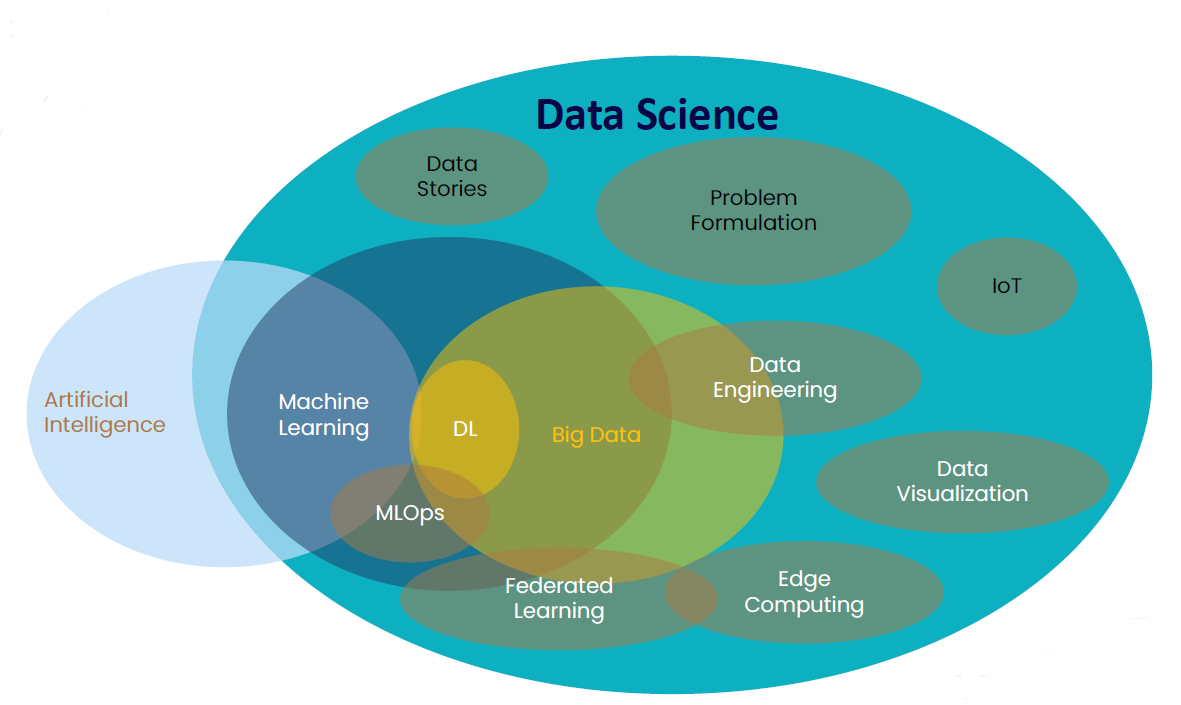
\includegraphics{Introduction to MLOps_files/mediabag/Venn_diagram.png}

}

\caption{Venn diagram of different domains under data science, and AI}

\end{figure}%

\subsection{Motivation for MLOps: Unlocking the potential of Machine
Learning
system}\label{motivation-for-mlops-unlocking-the-potential-of-machine-learning-system}

In the last ten years, machine learning has revolutionised many
industries, enabling automation, streamlining processes, and providing
insights which has flourished the companies. But as industries has
started incorporating machine learning into their operations at a large
scale, it has raised many complexities, few of which are how to
guarantee that a trained model is deployed in a production environment
without any problems? How to manage the lifecycle of numerous models to
ensure they remain precise and up-to-date? How to assure the close-knit
collaboration between data scientists, data engineers, business
managers, software engineers, and other stakeholders to ensure that
hand-offs occur efficiently, from data preparation and model training to
model deployment and monitoring? Are the machine learning models are
effectively offering the best business decisions? MLOps addresses all
that and then more.

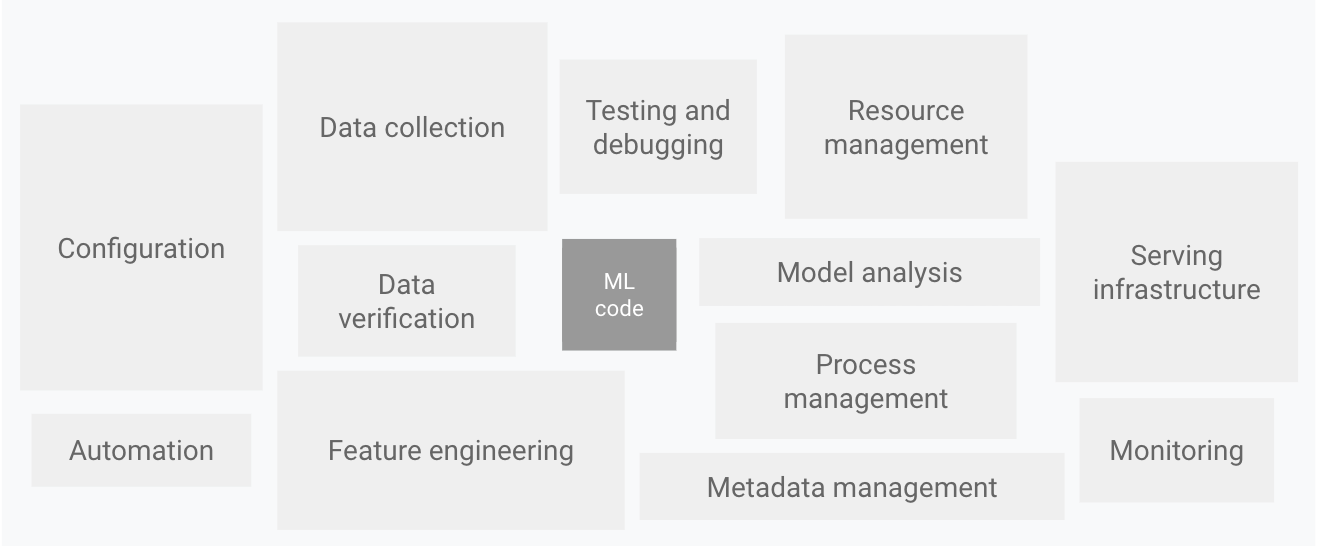
\includegraphics{Introduction to MLOps_files/mediabag/mlops-continuous-del.png}
\emph{\href{https://cloud.google.com/architecture/mlops-continuous-delivery-and-automation-pipelines-in-machine-learning}{Image
Source: Elements for ML systems}}

Teams at Google have been doing a lot of research on the technical
challenges that come with building ML-based systems. A NeurIPS paper on
hidden technical Debt in ML systems shows you developing models is just
a very small part of the whole process. There are many other processes,
configurations, and tools that are to be integrated into the system. To
streamline this entire system, we have this new Machine learning
engineering culture. The system involves everyone from the higher
management with minimal technical skills to Data Scientists to DevOps
and ML Engineers.

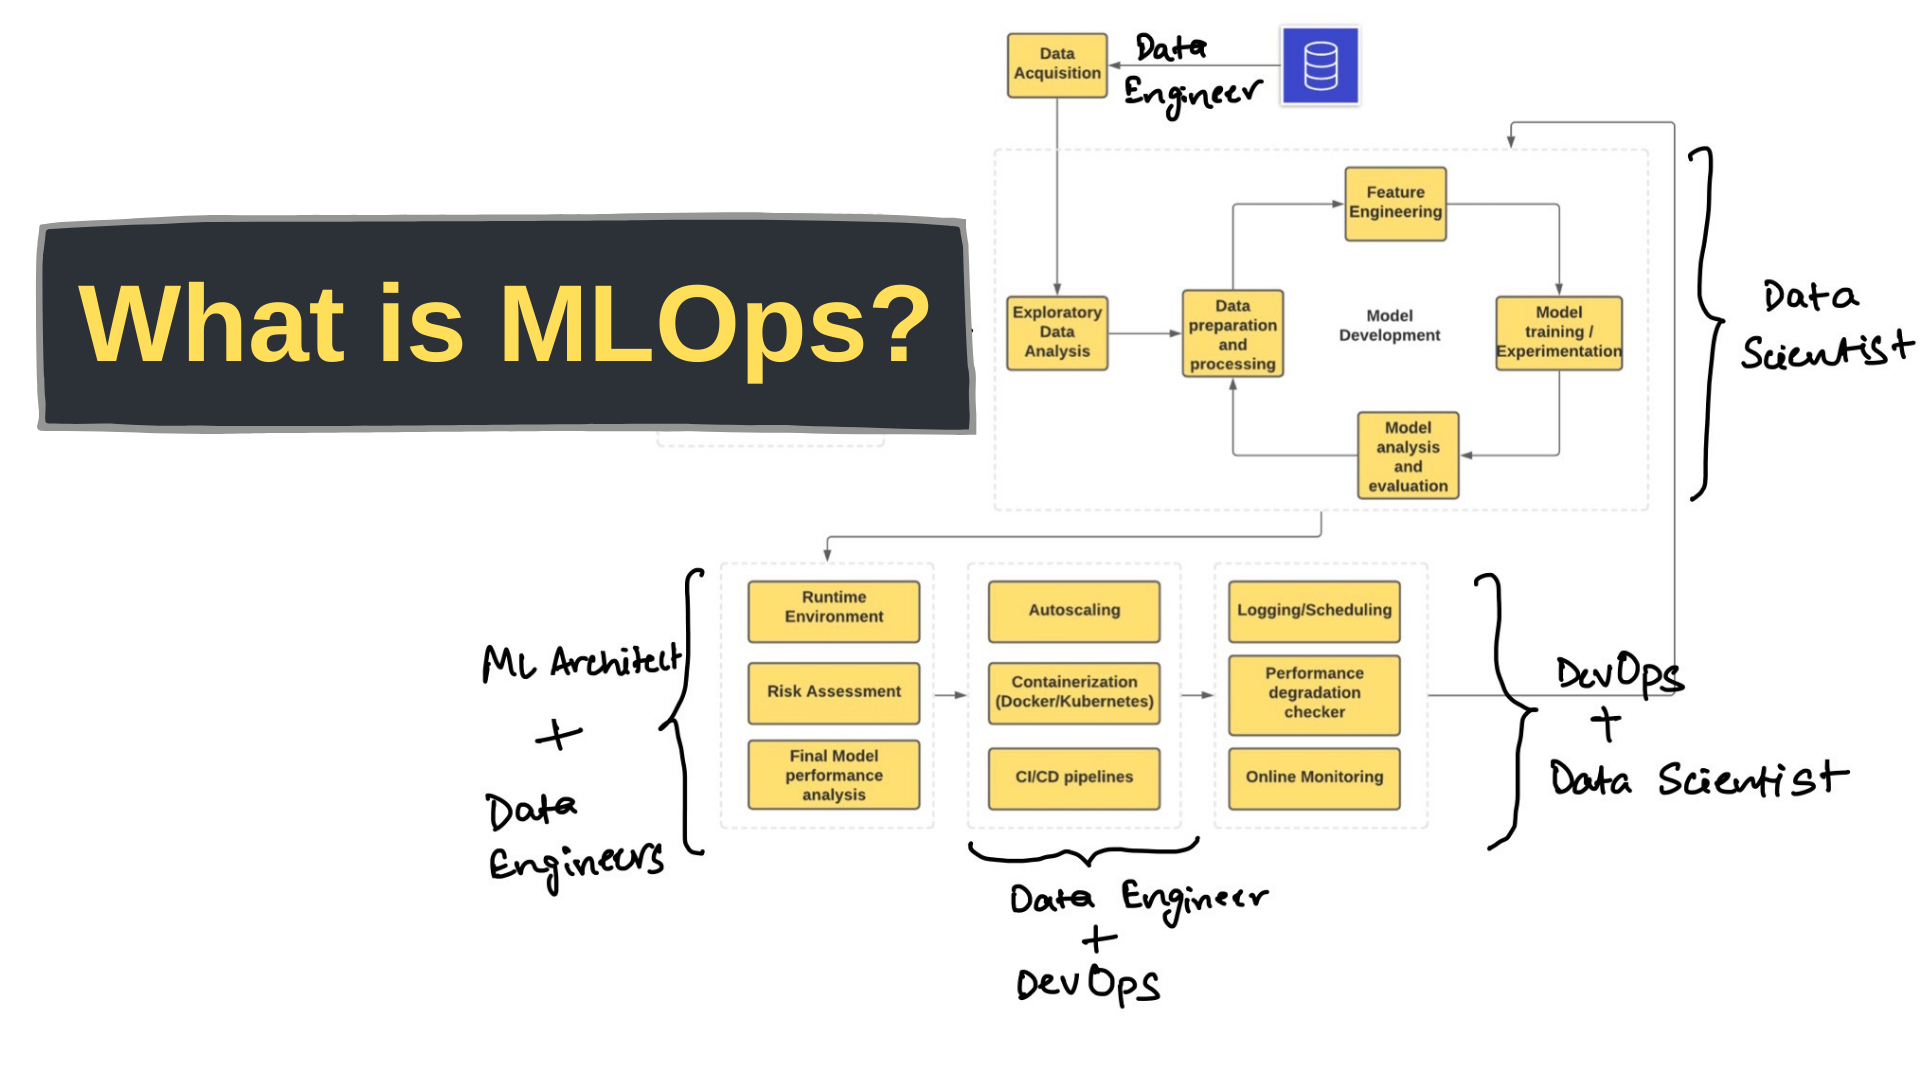
\includegraphics{Introduction to MLOps_files/mediabag/mlops_thumb.png}
\emph{\href{https://www.freecodecamp.org/news/what-is-mlops-machine-learning-operations-explained/}{Image
Source: What is MLOps?}}

\subsection{Differences Between Traditional Software systems and Machine
Learning
systems}\label{differences-between-traditional-software-systems-and-machine-learning-systems}

In the realm of software development, traditional software systems and
Machine Learning (ML) systems differ fundamentally despite some
overlaps. They differ in their approach to problem-solving, development
process, implemented and managed. Here are some key differences:

\begin{enumerate}
\def\labelenumi{\arabic{enumi}.}
\tightlist
\item
  \textbf{Problem Scope}:

  \begin{itemize}
  \tightlist
  \item
    \textbf{Traditional Software}: The problem, solution, and success
    metrics are clear from the beginning. For example, creating a
    marketplace for home rentals has a defined goal and success is a
    working platform {[}1{]}.
  \item
    \textbf{ML Systems}: The problem and solution may be unclear at the
    start and can change as the project progresses. Success is often
    measured by the optimization of model metrics like accuracy or
    precision {[}1{]}.
  \end{itemize}
\item
  \textbf{Quality Dependency}:

  \begin{itemize}
  \tightlist
  \item
    \textbf{Traditional Software}: Quality depends on the code. Changes
    in data do not impact the functionality unless new business rules
    are needed {[}2{]}.
  \item
    \textbf{ML Systems}: Quality depends on input data and
    hyperparameter tuning. New data may require retraining the model to
    maintain or improve performance {[}2{]}.
  \end{itemize}
\item
  \textbf{Continuous Evolution}:

  \begin{itemize}
  \tightlist
  \item
    \textbf{Traditional Software}: A programmer writes explicit rules or
    instructions for the computer to follow {[}3{]}. Once developed and
    tested, traditional software typically does not need to evolve
    unless there is a change in requirements, a need for optimization,
    or detected bugs. Updates are predictable and often scheduled.
  \item
    \textbf{ML Systems}: Algorithms learn from data without explicit
    programming. Models improve over time with feedback {[}3{]}. ML
    models in ML systems often require continuous updating and
    retraining. This is due to factors such as evolving data, changing
    patterns, and the nonstationary nature of many real-world scenarios
    (i.e., the underlying distribution of the problem changes over
    time). \emph{Example}: A model that predicts stock prices will need
    regular updates due to the dynamic nature of financial markets.
  \end{itemize}
\item
  \textbf{Data Dependency}:

  \begin{itemize}
  \tightlist
  \item
    \textbf{Traditional Software}: Relies less on data and more on
    predetermined logic {[}3{]}. The functionality is mostly independent
    of external data. While it processes data, its core behavior does
    not change on the basis of the data it has processed in the past.
  \item
    \textbf{ML Systems}: Heavily reliant on data to draw decision logic
    {[}4{]}. The effectiveness of ML models is intrinsically tied to the
    quality, quantity, and relevance of the training data. An ML model's
    behavior is shaped by its past data, making it crucial to ensure
    high-quality data for training. \emph{Example}: A chatbot trained on
    a limited and poor quality dataset might give irrelevant answers,
    whereas one trained on a diverse and comprehensive dataset can
    provide more accurate and context-aware responses.
  \end{itemize}
\item
  \textbf{Validation and Testing}:

  \begin{itemize}
  \tightlist
  \item
    \textbf{Traditional Software}: The functionality is mostly
    independent of external data. While it processes data, its core
    behavior does not change on the basis of the data it has processed
    in the past.
  \item
    \textbf{ML Systems}: The effectiveness of ML models is intrinsically
    tied to the quality, quantity, and relevance of the training data.
    An ML model's behavior is shaped by its past data, making it crucial
    to ensure high-quality data for training. \emph{Example}: A chatbot
    trained on a limited and poor quality dataset might give irrelevant
    answers, whereas one trained on a diverse and comprehensive dataset
    can provide more accurate and context-aware responses.
  \end{itemize}
\item
  \textbf{Outcome Predictability}:

  \begin{itemize}
  \tightlist
  \item
    \textbf{Traditional Software}: Exhibits deterministic behavior with
    predictable outcomes based on the given input{[}3{]}. For a given
    input, they will always produce the same output, provided the system
    state and configuration remain unchanged. Their behavior is
    explicitly programmed, meaning that developers define a set of rules
    and conditions that dictate the software's response to various
    inputs.
  \item
    \textbf{ML Systems}: Outcomes are probabilistic and can vary
    depending on the data it was trained on {[}3{]}. They generate
    outputs based on patterns identified during training. Consequently,
    they might produce different outcomes for slightly varying inputs,
    and there is inherent uncertainty in their predictions.
  \end{itemize}
\end{enumerate}

In summary, traditional software operates on a set of clear rules and is
less dependent on data, whereas ML systems are designed to learn from
data, requiring continuous improvement and adaptation to evolving data.
This fundamental difference impacts how problems are defined, how
success is measured, and how the systems are developed and maintained.

\subsection{Components of a ML system}\label{components-of-a-ml-system}

ML systems are intricate, with many workflows intertwined, many
stakeholders collaborating to convert raw data into useful predictions
or insights. It is essential to comprehend these components to create
and execute reliable ML solutions.

\begin{figure}[H]

{\centering 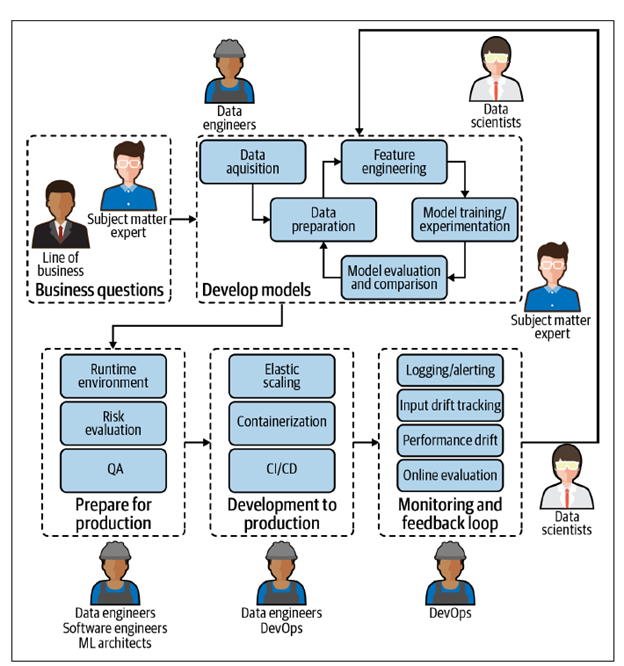
\includegraphics{Introduction to MLOps_files/mediabag/Picture_2.png}

}

\caption{The realistic picture of an ML model life cycle}

\end{figure}%

\emph{\href{https://www.oreilly.com/library/view/what-is-mlops/9781492093626/ch01.html}{Image
Source: What Is MLOps? by Mark Treveil, Lynn Heidmann}}

\begin{enumerate}
\def\labelenumi{\arabic{enumi}.}
\tightlist
\item
  \textbf{Data Acquisition:}\\
  The process of acquiring data from different sources, importing them,
  read and make them accessible for further workflows in the ML system.
  The key aspects are:
\end{enumerate}

\begin{itemize}
\tightlist
\item
  \textbf{Sources:} Data can be ingested from a variety of sources,
  including databases, data lakes, APIs, and streaming platforms.
\item
  \textbf{Formats:} Data can come in multiple formats such as CSV,
  Parquet, JSON, images, and more.
\item
  \textbf{Real-time vs.~Batch:} While real-time ingestion processes data
  as it's generated, batch ingestion involves processing data at
  intervals.
\end{itemize}

\begin{enumerate}
\def\labelenumi{\arabic{enumi}.}
\setcounter{enumi}{1}
\tightlist
\item
  \textbf{Data Preparation} At this stage, data from the previous stage
  is transformed from raw data into a format suitable for training ML
  models. The key aspects include:
\end{enumerate}

\begin{itemize}
\tightlist
\item
  \textbf{Cleaning:} Handling missing values, removing outliers, and
  correcting erroneous data.
\item
  \textbf{Feature Engineering:} Creating new features from existing ones
  to improve model performance.
\item
  \textbf{Normalization \& Scaling:} Adjusting the feature scales to
  ensure consistent model training.
\item
  \textbf{Encoding:} Converting categorical variables into numerical
  formats for the model.
\item
  \textbf{Data Augmentation (for image data):} Creating new training
  samples by applying transformations (e.g., rotation, flipping) to
  existing images.
\end{itemize}

\begin{enumerate}
\def\labelenumi{\arabic{enumi}.}
\setcounter{enumi}{2}
\tightlist
\item
  \textbf{Model Training} The core process where data is fed into
  algorithms to develop predictive models. The key aspects include:
\end{enumerate}

\begin{itemize}
\tightlist
\item
  \textbf{Algorithm Selection:} Choosing the right machine learning or
  deep learning algorithm for the problem.
\item
  \textbf{Hyperparameter Tuning:} Optimizing model parameters to enhance
  performance.
\item
  \textbf{Training Loops:} Iteratively updating the model weights based
  on the prediction error.
\item
  \textbf{Validation:} Using a separate data set to avoid overfitting
  and ensure the model generalizes well.
\end{itemize}

\begin{enumerate}
\def\labelenumi{\arabic{enumi}.}
\setcounter{enumi}{3}
\tightlist
\item
  \textbf{Model Evaluation} The process of assessing the performance of
  an ML model.The key aspects include:
\end{enumerate}

\begin{itemize}
\tightlist
\item
  \textbf{Metrics:} Depending on the problem type, different metrics are
  used (e.g., accuracy, precision, recall, F1 score for classification;
  MSE or RMSE for regression).
\item
  \textbf{Confusion Matrix:} A table used to evaluate classification
  models by comparing actual vs.~predicted classes.
\item
  \textbf{Cross-Validation:} A technique where the training set is split
  multiple times to assess the robustness of the model.
\item
  \textbf{AUC-ROC:} A grpahical representation for the performance of
  the classification model
\end{itemize}

\begin{enumerate}
\def\labelenumi{\arabic{enumi}.}
\setcounter{enumi}{4}
\tightlist
\item
  \textbf{Model Serving} Deploying trained models to make predictions on
  new data involves several key aspects:
\end{enumerate}

\begin{itemize}
\tightlist
\item
  \textbf{Deployment Platforms}: Models can be deployed on various
  platforms, including cloud services, on-premises servers, and edge
  devices.
\item
  \textbf{API Endpoints}: Models are exposed as services with API
  endpoints. These endpoints allow querying the model for predictions.
\item
  \textbf{Batch vs.~Real-Time Serving}:

  \begin{itemize}
  \tightlist
  \item
    \textbf{Batch Serving}: Provides predictions on bulk data all at
    once.
  \item
    \textbf{Real-Time Serving}: Offers immediate predictions for each
    input.
  \end{itemize}
\end{itemize}

\begin{enumerate}
\def\labelenumi{\arabic{enumi}.}
\setcounter{enumi}{5}
\tightlist
\item
  \textbf{Model Monitoring} Continuously observing and analyzing
  deployed models' behavior and performance is crucial. Here are the key
  aspects of model monitoring:
\end{enumerate}

\begin{itemize}
\tightlist
\item
  \textbf{Performance Monitoring}: Track accuracy, latency, and other
  relevant metrics after deployment. Ensure the model performs as
  expected.
\item
  \textbf{Logging}: Keep records of prediction requests, responses, and
  errors. Useful for debugging and auditing.
\item
  \textbf{Alerts}: Set up automatic notifications for anomalies or
  performance degradations. Prompt action when issues arise.
\item
  \textbf{Model Drift Detection}: Monitor data distribution over time.
  Detect changes that may impact model performance.
\end{itemize}

\subsection{Key Components of MLOps}\label{key-components-of-mlops}

\subsubsection{1. Continuous Integration \& Continuous Deployment
(CI/CD)}\label{continuous-integration-continuous-deployment-cicd}

CI/CD pipelines automate the process of building, testing, and deploying
ML models. This ensures that changes to models or code are quickly
integrated and deployed into production environments.

\includegraphics{Introduction to MLOps_files/mediabag/CI_CD-Pipeline.f94b9.png}
\emph{Image Source: Amazon Web Services}

\subsubsection{2. Model Versioning \&
Registry}\label{model-versioning-registry}

Model versioning and registry systems track and manage different
versions of ML models, making it easy to rollback changes if necessary
and ensuring reproducibility of experiments.

\includegraphics{Introduction to MLOps_files/mediabag/1-bKFfJbtpCUBb0VJ2R9.png}
\emph{Image Source: Medium}

\subsubsection{3. Model Monitoring \&
Observability}\label{model-monitoring-observability}

Monitoring and observability tools track the performance of deployed
models in real-time, detecting drift, anomalies, and degradation in
model accuracy, and triggering alerts for corrective actions.

\includegraphics{Introduction to MLOps_files/mediabag/Production-Monitorin.png}
\emph{Image Source: Databricks}

Steps in the MLOps process

Where MLOps sees the biggest benefit is in the iterative orchestration
of tasks. While data scientists are reviewing new data sources,
engineers are adjusting ML configurations. Making simultaneous
adjustments in real-time vastly reduces the time spent on improvements.

\subsection{Benefits of MLOps}\label{benefits-of-mlops}

\subsubsection{Reducing Time-to-Market}\label{reducing-time-to-market}

\begin{itemize}
\item
  \emph{\textbf{Rapid Prototyping}}: MLOps allows teams to quickly
  iterate over models, helping them move from conceptualization to
  deployment swiftly.
\item
  \emph{\textbf{Automation}}: Automated pipelines reduce manual errors
  and speed up repetitive tasks like data pre-processing, model
  validation, and deployment.
\item
  \emph{\textbf{Feedback Loops}}: Faster model training and deployment
  cycles enable organizations to get faster feedback, aiding in timely
  model adjustments.
\end{itemize}

\subsubsection{Ensuring Model Reliability and
Robustness}\label{ensuring-model-reliability-and-robustness}

\begin{itemize}
\item
  \emph{\textbf{Reproducibility}}: MLOps emphasizes versioning not just
  for code but also for data and model configurations, ensuring that
  experiments are reproducible.
\item
  \emph{\textbf{Continuous Evaluation}}: With continuous monitoring,
  models are regularly evaluated against new data to detect and address
  perfor- mance degradation.
\item
  \emph{\textbf{Alert Mechanisms}}: MLOps tools can raise instant alerts
  if a model's performance dips below a threshold or if anomalies are
  detected, ensuring timely interventions.
\end{itemize}

\subsubsection{Simplifying Model
Management}\label{simplifying-model-management}

\begin{itemize}
\item
  \emph{\textbf{Centralized Model Registry}}: MLOps practises often
  include main- taining a centralised model registry where all models,
  their ver- sions, and metadata are stored, simplifying model discovery
  and management.
\item
  \emph{\textbf{Rollbacks and Canary Deployments}}: If a newly deployed
  model fails, MLOps enables swift rollbacks to the previous stable
  version. Canary deployments allow one to test new models on a fraction
  of the traffic before a full-scale rollout.
\item
  \emph{\textbf{Scalability}}: MLOps infrastructure is designed to
  scale, ensuring that the models can handle varying loads, from a few
  requests per sec- ond to thousands.
\end{itemize}

\subsubsection{Ensuring Regulatory and Ethical
Compliance}\label{ensuring-regulatory-and-ethical-compliance}

\begin{itemize}
\item
  \emph{\textbf{Audit Trails}}: MLOps tools log every action, change,
  and decision made in the ML workflow, enabling traceability and
  satisfying reg- ulatory requirements.
\item
  \emph{\textbf{Bias Detection and Fairness Checks}}: MLOps emphasises
  continuous monitoring for biases and unfair decision-making, helping
  organi- sations uphold ethical standards and avoid reputational risks.
\item
  \emph{\textbf{Data Security and Privacy}}: With the increasing
  importance of data in ML workflows, MLOps ensures that data are
  stored, accessed, and used securely, respecting privacy norms and
  regulations.
\end{itemize}

In conclusion, MLOps plays a crucial role in enabling organizations to
operationalize and scale their machine learning initiatives effectively.
By integrating best practices from software engineering and data
science, MLOps fosters collaboration, agility, and reliability in the
development and deployment of ML solutions.

\subsection{How generative AI is evolving
MLOps}\label{how-generative-ai-is-evolving-mlops}

The release of OpenAI's ChatGPT sparked interests in AI capabilities
across industries and disciplines. This technology, known as generative
AI, has the capability to write software code, create images and produce
a variety of data types, as well as further develop the MLOps process
{[}7{]}.

Generative AI is a type of deep-learning model that takes raw data,
processes it and ``learns'' to generate probable outputs. In other
words, the AI model uses a simplified representation of the training
data to create a new work that's similar, but not identical, to the
original data. For example, by analyzing the language used by
Shakespeare, a user can prompt a generative AI model to create a
Shakespeare-like sonnet on a given topic to create an entirely new work.

Generative AI relies on foundation models to create a scalable process.
As AI has evolved, data scientists have acknowledged that building AI
models takes a lot of data, energy and time, from compiling, labeling
and processing data sets the models use to ``learn'' to the energy is
takes to process the data and iteratively train the models. Foundation
models aim to solve this problem. A foundation model takes a massive
quantity of data and using self-supervised learning and transfer
learning can take that data to create models for a wide range of tasks
{[}7{]}.

This advancement in AI means that data sets aren't task specific---the
model can apply information it's learned about one situation to another.
Engineers are now using foundation models to create the training models
for MLOps processes faster. They simply take the foundation model and
fine-tune it using their own data, versus taking their data and building
a model from scratch {[}7{]}.

\subsection{Citations}\label{citations}

\begin{enumerate}
\def\labelenumi{\arabic{enumi}.}
\tightlist
\item
  {[}What is MLOps? Machine Learning Operations Explained{]} - Source:
  \href{https://www.freecodecamp.org/news/what-is-mlops-machine-learning-operations-explained/}{FreeCodeCamp}
\item
  {[}How machine learning differs from traditional-software{]} - Source:
  \href{https://medium.com/machine-learning-in-practice/how-machine-learning-differs-from-traditional-software-80d0a235ff3b}{Medium}
\item
  {[}difference between machine learning traditional software{]}-
  Source:
  \href{https://vitalflux.com/difference-between-machine-learning-traditional-software/}{vitalflux}
\item
  {[}Traditional Programming vs Machine Learning{]}- Source:
  \href{https://insightsoftware.com/blog/machine-learning-vs-traditional-programming/}{insightsoftware}
\item
  {[}Test \& Evaluation Best Practices for Machine Learning-Enabled
  Systems{]}- Source: \href{https://arxiv.org/pdf/2310.06800}{arxiv}
\item
  {[}Introduction to MLOps{]}- Source:
  \href{https://readmedium.com/en/https:/ogre51.medium.com/introduction-to-mlops-815d03c8a4d4}{Medium:ogre51}
\item
  {[}MLOps and the evolution of data science{]}- Source:
  \href{https://www.ibm.com/blog/mlops-and-the-evolution-of-data-science/}{IBM}
\end{enumerate}



\end{document}
